\chapter{Zenbakizko Integratzaile Sinplektikoak.}

\section{Sarrera.}

\subsection{Zenbakizko metodoak.}

Ekuazio diferentzial arruntetarako (\emph{ODE}) hasierako baliodun problemen (\emph{IVP}) formulazioa,
\begin{equation}
\label{eq:21}
\dot{\mathbf{y}}(t)=\mathbf{f}(t,\mathbf{y}(t)),\ \ \ \mathbf{y}(t_0)=\mathbf{y_0}, 
\end{equation}
non  $\bf{y}: \mathbb{R} \longrightarrow {\mathbb{R}}^d$ soluzioa, $\bf{y_0} \in \mathbb{R}^d$ hasierako balioa eta $\bf{f}: \ \mathbb{R} \times {\mathbb{R}}^d \ \longrightarrow {\mathbb{R}}^d$ bektore eremua deskribatzen funtzioa dugun ($\dot{\mathbf{y}}$ notazioa erabiliko dugu $d\mathbf{y}/dt$ adierazteko).

\paragraph*{} $t_0$ unetik $t_0+h$ integrazioa,
\begin{equation*}
\mathbf{y}(t_0+h)=\mathbf{y_o}+\int\limits_{t_0}^{t_0+h} \mathbf{f}(t,\mathbf{y}(t)) dt.
\end{equation*}

\paragraph*{}Goiko ekuazio-sistema bektoriala (\ref{eq:21}), ekuazio-sistema modu eskalarrean idatzi daiteke:

\[\dot{y_1}(t)=f_1(t,(y_1(t),y_2(t),\dots,y_d(t)), \ \ y_1(t_0)=y_{1,0}\]
\[\dot{y_2}(t)=f_2(t,(y_1(t),y_2(t),\dots,y_d(t)), \ \ y_2(t_0)=y_{2,0}\]
\[\dots\]
\[\dot{y_d}(t)=f_d(t,(y_1(t),y_2(t),\dots,y_d(t)),  \ \ y_d(t_0)=y_{d,0}\]


\paragraph*{} Metodo analitikoak (funtzio ezagunen araberako soluzio zehatza) eta erdi-analitikoak, ez dira problema askoren soluzioa bilatzeko teknika egokiak. Zenbakizko metodoak, aldiz, modu errazean aplika daitezke eta horregatik, soluzio metodo nagusiena kontsideratzen da. 

\paragraph*{}Zenbakizko metodo baten bidez, $\mathbf{y}(t)$ soluzioaren $\mathbf{y_n} \approx \mathbf{y}(t_n)$ hurbilpena lortuko dugu $t_n=t_{n-1}+h_n$  ($n=1,2,\dots$)  une diskretu ezberdinetarako. Zenbakizko soluzioa urratsez-urrats sekuentzialki eta zehaztutako tarte baterako ($t_0\le t \le t_f$) kalkulatuko dugu. Beraz, lortutako balio  multzoak $(t_o,\mathbf{y_0}),(t_1,\mathbf{y_1}),\dots,(t_f,\mathbf{y_f})$ zenbakizko soluzioa definitzen du.   

\paragraph*{} Nola jakin zenbakizko soluzioa matematika modeloarekiko zuzena dela? Zenbakizko soluzioaren errorea neurtzeko teknika ezberdinak ditugu.           

\paragraph*{} Azkenik argitu beharra dago ekuazio-sistema beti \emph{sistema autonomo} moduan, hau da, denborarekiko independentea idatz daitekeela. Hori horrela izanik, notazioa sinplifikatzeko era honetako sistemak kontsideratuko ditugu,   

\begin{equation}
%\label{eq:31}
\dot{\mathbf{y}}(t)=\mathbf{f}(\mathbf{y}(t)),\ \ \ \mathbf{y}(t_0)=\mathbf{y_0}.
\end{equation}


\paragraph*{}Jarraian zenbakizko metodoen oinarrizko kontzeptuak eta notazioa finkatuko dugu.

\begin{enumerate}

\item Fluxua.

Fase-espazioko edozein $\mathbf{y_0}$ puntuari, $\mathbf{y}(t_0)=\mathbf{y_0}$ hasierako balio duen $\mathbf{y}(t)$ soluzioa asignatzen dion mapping-ari deitzen diogu. Izendatzeko $\varphi_t$ notazioa erabiliko dugu,
\begin{equation*}
\varphi_t(\mathbf{y_0})=\mathbf{y}(t) \ \ \text{baldin} \  \mathbf{y}(t_0)=\mathbf{y_0}
\end{equation*}

\item Zenbakizko diskretizazioa.

$\mathbf{y_{n}},\mathbf{y_{n-1}},\dots ,\mathbf{y_0}$ balioak emanda, $\mathbf{y_{n+1}}\approx \mathbf{y}(t_{n+1})$ soluzioaren hurbilpena kalkulatzeko formulari \emph{zenbakizko fluxua} deritzogu. Honako notazioa erabiliko dugu,
\begin{equation*}
\mathbf{y_{n+1}}=\phi(\mathbf{y_{n+1}},\mathbf{y_{n}},\dots,\mathbf{y_0};h;f).
\end{equation*}

$\phi$ metodoa, $\mathbf{y_{n+1}}$ balioaren menpe ez dagoenean, $\mathbf{y_{n+1}}$ zuzenean kalkula daiteke eta metodoa \emph{esplizitua} dela esaten zaio. Aldiz, $\phi$ metodoa $\mathbf{y_{n+1}}$ menpe dagoenean, $\mathbf{y_{n+1}}$ askatzeko zeharkako bidea erabili behar da (adibidez Newton sinplifikatua edo puntu finkoaren metodoa) eta metodoari \emph{inplizitua} dela esaten zaio.  

\paragraph*{} Adibideak.

Eurler metodo esplizitua.
\begin{equation*}
\label{eq41}
\mathbf{y_{n+1}}=\mathbf{y_n}+h  \ \mathbf{f}(\mathbf{y_n}) 
\end{equation*} 

Eurler metodo inplizitua.
\begin{equation*}
\label{eq41}
\mathbf{y_{n+1}}=\mathbf{y_n}+h  \ \mathbf{f}(\mathbf{y_{n+1}}) 
\end{equation*} 

\item Metodoaren ordena.

\paragraph*{}Definizioa. \textbf{Errore globala}. Zenbakizko soluzioaren $t_0$ hasierako unetik $t_k$ une arteko errore globala $ge(t)$,
\begin{equation*}
ge(t_k)=y_k-y(t_k).
\end{equation*}
  
\paragraph*{} Definizioa. \textbf{$\mathbf{\phi}$ metodoaren ordena}. $h$ urrats luzera finkoko $\phi$ metodoak $p$ ordenekoa dela esaten da, errore globala $ge(t)$  $O(h^{p})$ ordenekoa bada  $h \rightarrow 0$,
\begin{equation*}
y_k-y(t_k)=O(h^{p}), \ \ h \rightarrow 0.
\end{equation*}   

\paragraph*{}Definizioa. \textbf{Errore lokala}. Zenbakizko soluzioaren urrats bakarreko $[t_k,t_{k+1}]$ errore lokala $le(t)$,
\begin{equation*}
le(t_{k+1})=y_{k+1}-y_k(t_{k+1})
\end{equation*}  
non $y_k(t)$, $y(t_k)=y_k$ hasierako balio lokaleko soluzio zehatza den. 

Metodoaren ordena $O(h^p)$ bada, errore lokala $O(h^{p+1})$ da.

\item  Metodo simetrikoak.

\paragraph*{\textbf{Adjoint method}.} Jatorrizko metodoaren alderantzizko eta kontrako denbora $-h$ esleipenari (map), $\phi_h$ metodoaren $\phi_h^{*}$ \emph{adjoint metodoa} esaten zaio.

\begin{equation*}
\phi_h^{*}=\phi_{-h}^{-1}
\end{equation*}

$\phi_h^{*}=\phi_h$  --betetzen denean, metodoa simetrikoa da. 

\end{enumerate}


\subsection{Problema motak.}

\begin{enumerate}

\item Problema kaotikoak. 

Hasierako balio edo parametroen perturbazioekiko, diskretizazio-erroreekiko (trunkatze) edo birbitze erroreekiko esponentzialki sentikorrak diren problemei esaten zaie.

\item Problema stiff.

Irakurri $12.1$ Solution of stiff problems ($555-559$).

Irakurri $13.2.3$ Convergence and consistency and $13.3$ Stiffness and Implicitness (600).

\end{enumerate}


\subsection{Sistema-Hamiltondarrak.}


Ekuazio diferentzial arrunten (EDA) formulazio Hamiltondarra erabili ohi da errealitateko sistemak matematikoki adierazteko. Azpimarratu metodo sinpletikoak sistema Hamiltondar hauen soluzioaren hurbilpena kalkulatzeko zenbakizko metodo bereziki onak ditugula. 

\paragraph*{} $H(\mathbf{p},\mathbf{q})$ funtzio leuna izanik, non  $H: \ {\mathbb{R}}^{d} \ \longrightarrow {\mathbb{R}}$  eta  $(\mathbf{p},\mathbf{q})=(p_1, \dots , p_n,q_1, \dots , q_n)$ ($d=2n$),  dagokion ekuazio diferentzialak era honetan definitzen dira,

\begin{equation}\label{eq:11}
\frac{d}{dt}{p}_j=-\frac{\partial H(\mathbf{p},\mathbf{q})}{\partial q_j}, \ \ \frac{d}{dt}{q}_j=\frac{\partial H(\mathbf{p},\mathbf{q})}{\partial p_j}, \ \ \ \ j=1,\dots,n.
\end{equation} 

Edo notazio laburtua erabiliz,

\begin{equation}
\dot{\mathbf{y}}=J^{-1}\triangledown H(\mathbf{y}),\ \ 
y=\left(\begin{array}{c}
  p \\
  q \\
  \end{array}\right), \ \
J=\left(\begin{array}{cc}
  \ 0 & \ I \\
   -I & \ 0 \\
\end{array}\right),  
\end{equation}

\paragraph*{}$\mathbf{p}$ eta $\mathbf{q}$ bektoreen $n$ dimentsioa sistemaren \emph{askatasun maila} deritzo. $H(\mathbf{p},\mathbf{q})$ funtzioaren balioa integrazioan zehar konstante mantentzen da.

\subsubsection*{Adibidea.} Penduluaren problemaren (masa $m=1$, $l=1$ luzerako makila eta $g=1$ grabitazioa) askatasun bakarreko sistema Hamiltondarra,

\begin{equation*}
H(p,q)=\frac{1}{2} p^2- cos q.
\end{equation*}

Ekuazio diferentzialak,
\begin{equation*}
\dot{p}= -sin q, \ \ \dot{q}=p.
\end{equation*}

\begin{figure}[h]
\centering
\subfloat[Pendulua.]{
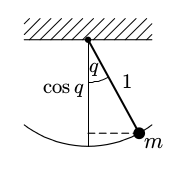
\includegraphics[width=.250\textwidth]{SinglePendulum}
}
\caption{ \small Pendulua.}
\label{fig:pendulua}
\end{figure}

\subsubsection*{Hamiltondar banagarriak.}

Hamiltondar banagarriak egitura bereziko sistema Hamiltondarrak ditugu. Sistema-mekanikoak era honetako Hamiltondarra dute $H(\mathbf{p},\mathbf{q})=T(\mathbf{p})+U(\mathbf{q})$.

Horien artean, \emph{bigarren ordeneko} ekuazio diferentzialak aipatu behar ditugu, zeintzuk Hamiltondar banagarri kasu partikularra bat diren,  

\begin{equation*}
H(\mathbf{p},\mathbf{q})=\frac{1}{2}\mathbf{p}^T\mathbf{p} +U(\mathbf{q}).
\end{equation*}

Beraz, dagokien ekuazio diferentzialak,
\begin{equation*}
\dot{\mathbf{p}}=-\frac{\partial U(\mathbf{q})}{\partial \mathbf{q}}, \ \ \dot{\mathbf{q}}=\mathbf{p}. 
\end{equation*}

\subsubsection*{Adibidea.}
\emph{Bi-gorputzen problema} edo \emph{Kepler problema}. Planoan elkar erakartzen diren bi gorputzen (planeta eta eguzkia) mugimendua kalkulatzeko, horietako gorputz baten kokapena koordenatu sistemaren jatorria kontsideratuko dugu eta beste gorputzaren kokapenaren koordenatuak $\mathbf{q}=(q_1,q_2)$ aukeratuko ditugu. Normalizatutako Newton legearen araberako ekuazio diferentzialak,  

\begin{equation}
\dot{p}_1= -\frac{q_1}{(q_1^2+q_2^2)^{3/2}}, \ \, \dot{p}_2= -\frac{q_2}{(q_1^2+q_2^2)^{3/2}}.
\end{equation}
  
\begin{equation}
\dot{q}_i=p_i, \ \ i=1,2.
\end{equation}

Baliokide den sistema Hamiltondarra,
\begin{equation}
H(p_1,p_2,q_1,q_2)=\frac{1}{2}(p_1^2+p_2^2)-\frac{1}{\sqrt{q_1^2+q_2^2}}.
\end{equation}

\paragraph*{} Planetaren mugimendua orbita eliptiko bat da. Honako hasierako balioei dagokien soluzioa,
\begin{equation*}
q_1(0)=1-e, \ q_2(0)=0, \ p_1(0)=0, \ p_2(0)=\sqrt{ \frac{1+e}{1-e}}, 
\end{equation*}
$e$ ezentrizidade ($0\le e < 1$) duen elipsea da, eta $P=2\pi$ periododuna. 
 
\subsubsection*{Hamiltondar perturbatuak.}

Hamiltondar perturbatuak, honako egitura duten,

\begin{equation*}
H=H_A+\epsilon H_B \ \ (|H_B|\ll |H_A|),
\end{equation*}

sistemak ditugu. Adibidez Eguzki sistemaren probleman, Hamiltondarra modu honetan idatzi daiteke $H=H_k+H_I$, non alde nagusia $H_K$ planeta bakoitzaren eguzki inguruko mugimendu kepleriarra den eta $H_I$ aldiz, planeten arteko interakzioek eragiten duten perturbazio txikia.   

Eguzki-sistemaren kasuan, \emph{Jakobi} koordenatuak erabiliz Hamiltondarra $H(\mathbf{p},\mathbf{q})=H_K(\mathbf{p},\mathbf{q})+H_I(\mathbf{q})$ moduan banatzen da, non $H_K(\mathbf{p},\mathbf{q})$ Kepler problema independenteak eta $H_I(\mathbf{q})$ integratu daitezkeen. Beste aukera, koordenatu \emph{Heliozentrikoak} erabiliz $H(\mathbf{p},\mathbf{q})=H_K(\mathbf{p},\mathbf{q})+H_I(\mathbf{p},\mathbf{q})$ moduan banatzen da, non $H_I(\mathbf{p},\mathbf{q})$ ezin daitekeen zuzenean integratu.

\section{Metodo sinplektikoak.}

\paragraph*{} Urrats luzera. Metodo gehienak eraginkorrak izateko, errore estimazio baten arabera integrazioan zehar urrats luzera egokitzen dute. Integratzaile sinplektikoetan, urrats luzeera finkoa erabili behar da metodoaren propietateak ez galtzeko.  

\paragraph{\textbf{Implicit midpoint}.}

\begin{equation*}
p_{n+1}=p_n-h \triangledown_q H(\frac{p_{n+1}+p_n}{2},\frac{q_{n+1}+q_n}{2})
\end{equation*}

\begin{equation*}
q_{n+1}=q_n+h \triangledown_p H(\frac{p_{n+1}+p_n}{2},\frac{q_{n+1}+q_n}{2})
\end{equation*}

\paragraph*{\textbf{Störmer-Verlet  metodoa}.}
$p=2$ ordeneko metodo sinplektikoa eta simetrikoa dugu.

\[p_{\frac{n+1}{2}}=p_n-\frac{h}{2} \triangledown_q H(p_{\frac{n+1}{2}},q_n) \]
\begin{equation}
q_{n+1}=q_n+\frac{h}{2} \big(\triangledown_p H(p_{\frac{n+1}{2}},q_n)+ \triangledown_p H(p_{\frac{n+1}{2}},q_{n+1}) \big)
\end{equation}
\[p_{n+1}=p_{\frac{n+1}{2}}-\frac{h}{2} \triangledown_q H(p_{\frac{n+1}{2}},q_{n+1}) \]

edo

\[q_{\frac{n+1}{2}}=q_n+\frac{h}{2} \triangledown_p H(p_n,q_{\frac{n+1}{2}}) \]
\begin{equation}
p_{n+1}=p_n-\frac{h}{2} \big(\triangledown_q H(p_n,q_{\frac{n+1}{2}})+ \triangledown_q H(p_{n+1},q_{\frac{n+1}{2}}) \big)
\end{equation}
\[q_{n+1}=q_{\frac{n+1}{2}}+\frac{h}{2} \triangledown_p H(p_{n+1},q_{\frac{n+1}{2}}) \]


\paragraph*{}Bigarren ordeneko ekuazio diferentziala ditugunean metodoa esplizitua da eta modu honetan labur daiteke,

\[p_{{n+1}/{2}}=p_n+\frac{h}{2} f(q_n)\]
\begin{equation}
q_{n+1}=q_n+h p_{{n+1}/{2}}
\end{equation}
\[p_{n+1}=p_{{n+1}/{2}}+\frac{h}{2}f(q_{n+1})\]

edo

\[q_{{n+1}/{2}}=q_n+\frac{h}{2} p_n\]
\begin{equation}
p_{n+1}=p_n+h f(q_{{n+1}/{2}})
\end{equation}
\[q_{n+1}=q_{{n+1}/{2}}+\frac{h}{2} p_{n+1}\]

\section{Gauss metodoak.}

\subsection{Runge-Kutta metodoak.}

Runge-Kutta metodoak, urrats bakarreko ekuazio diferentzial arrunten zenbakizko integratzaileak dira.  $b_{i}$, $a_{ij}$ eta $c_i=\sum\limits_{i=0}^{s} a_{ij} \ (1 \leq i,j \leq s)$ koefiziente errealek s-ataleko Runge-Kutta metodoa definitzen dute . \emph{Butcher} izeneko taulan moduan laburtu ohi dira koefiziente hauek, 

\begin{equation}
\begin{array}{c|c}
  \bf{c} & \bf{A} \\
  \hline
         &  \bf{b}^T\\
\end{array}, \ \ \ \ \ \ \ \ \ \ \ \
\begin{array}{c|cccc}
  \ c_1 &  a_{11} & a_{12} & \dots & a_{1s}\\
  \ c_2 &  a_{21} & a_{22} & \dots &a_{2s}\\
  \ \vdots & \vdots & \ddots & & \vdots \\
  \ c_s & a_{s1} & a_{s2} & \dots & a_{ss}\\
  \hline
  \  & b_{1} & b_{2} & \dots & b_{s}\\
\end{array}
\end{equation}

\paragraph*{} Hasierako baliodun problema (\ref{eq:21}) baten $\mathbf{y}(t)$ soluzioaren $\mathbf{y}_n \approx \mathbf{y}(t_n)$ hurbilpena era honetan kalkulatzen da,

\begin{equation}  
\mathbf{y}_{n+1}=\mathbf{y}_n+h\sum^s_{i=1}{b_i \ \mathbf{f}(\mathbf{Y}_{n,i})\ \ },\
\end{equation} 

non $\mathbf{Y}_{n,i}$ atalak era honetan definitzen diren,
\begin{equation}
\mathbf{Y}_{n,i}=\mathbf{y}_n+\ h\ \sum^s_{j=1}{a_{ij}\ \mathbf{f}(\mathbf{Y}_{n,j})}\ \ \ \ \ i=1 ,\dots, s.\
\end{equation} 

\subsubsection*{Metodo esplizituak (ERK) eta inplizituak (IRK).}
Bi mota nagusi bereizi ditzakegu: esplizituak (\emph {ERK}) non $\forall i\ge j, \ a_{ij}=0 $ eta inplizituak (\emph {IRK}) non $\exists i \ge j \ , a_{ij} \ne 0$ . \emph{ERK} metodoak problema Nonstiff-etarako eraginkorrak kontsideratzen dira eta \emph{IRK} metodoak ordea, problema Stiff-etarako.

\paragraph*{} Adibideak: ERK lau-ataletako metodo klasikoa (ezkerrekoa) and Implicit Midpoint method (eskuindekoa). 
\begin{equation}
\begin{array}{c|cccc}
  \ 0   &    &    &     &      \\
  \ 1/2 & 1/2 &   &     &      \\
  \ 1/2 & 0   & 1/2  &  &      \\
  \ 1   & 0   & 0    &  1   &   \\
  \hline
  \     & 1/6 & 2/6  &  2/6 & 1/6 \\
\end{array}, \ \ \ \ \ \ \ \ \ \ \ \
\begin{array}{c|c}
  \ 1/2 &  1/2\\
  \hline
  \     & 1 \\
\end{array} \\
\end{equation}

\paragraph*{}\emph{ERK} lau-ataletako  metodo klasikoa $p=4$ ordeneko dugu. Orden altuko \emph{ERK} metodoak aurkitzea konplexua da,  betearazi behar diren baldintza kopuru esponentzialki hazten baitira. Orden altuko \emph (ERK) metodo hauek aurkitu dira: $p=8$ ordeneko metodoa $s=11$ atalekin, $p=10$ ordeneko metodoa $s=17$ atalekin eta  $p=12$ ordeneko metodoa $s=25$ atalekin. 

\paragraph*{} \emph{IRK} metodoak \emph{ERK} metodoak baino modu errazagoan eraiki daitezke.  \emph{Butcher sinplifikazio baldintzen} \cite{Butcher2008} arabera definitzen dira,

\begin{equation*}
B(p): \ \ \ \sum\limits_{i=1}^{s} b_ic_i^{q-1}=\frac{1}{q}, \ \ q=1,\dots,p.
\end{equation*}

\begin{equation*}
C(\eta): \ \ \ \sum\limits_{j=1}^{s} a_{ij}c_j^{q-1}=\frac{c_i^q}{q}, \ \ i=1,\dots,s, \ q=1,\dots,\eta.
\end{equation*}

\begin{equation*}
D(\zeta):  \ \ \ \sum\limits_{i=1}^{s}  b_i c_i^{q-1}  a_{ij}  = \frac{b_j}{q} (1-c_j^q),  \ j=1,\dots,s, \ q=1,\dots,\zeta.
\end{equation*}

\begin{table}{htb}
\caption{Runge-Kutta metodo inplizituak.}
\label{tab:21}       % Give a unique label
\begin{tabular}{ c c c c c } 
 \hline
 Metodoa          &  Baldintzak             &                        &                 & Ordena \\
 \hline
 Gauss            &  $B(2s)$                & $C(s)$                 & $D(s)$          & $2s$    \\
 \hline
 Radau IA         &  $B(2s-1)$              & $C(s-1)$               & $D(s)$          & $2s-1$  \\
 \hline 
 Radau IA         &  $B(2s-1)$              & $C(s)$                 & $D(s-1)$        & $2s-1$  \\
 \hline 
 Lobatto IIIA     &  $B(2s-2)$              & $C(s)$                 & $D(s-2)$        & $2s-2$  \\
 \hline
 Lobatto IIIB     &  $B(2s-2)$              & $C(s-2)$               & $D(s)$          & $2s-2$  \\
 \hline 
 Lobatto IIIC     &  $B(2s-2)$              & $C(s-1)$               & $D(s-1)$        & $2s-2$  \\
  \hline
 \end{tabular}
\end{table}

\paragraph*{}Aurreko taulan (Taula \ref{tab:21}) \emph{IRK} metodo ezagunenak laburtu ditugu. Gauss metodoa s-ataletako IRK metodoen artean $p=2s$ ordena duen metodo bakarra dugu. Gauss metodoa sinplektikoa eta simetrikoa da.

\begin{enumerate}
\item{Sinplektizidade baldintza} \cite{JMSanz-Serna1994}.
\begin{equation} \label{eq:1}
b_{i}a_{ij}+b_{j}a_{ji}-b_{i}b_{j}=0, \ \ 1 \leqslant i,j \leqslant s
\end{equation}
%\cite{Sanz-Serna1992}.
 
\item{Koefiziente simetrikoak}.
 \begin{equation} \label {eq:2}
 b_{i} = b_{(s-i+1)} ,\ \  i=1,2,\dots \lceil s/2\rceil
 \end{equation} 
  \begin{equation} \label{eq:3}
 c_{(s-i+1)}= 1-c_{i}, \ \  i=1,2,\dots \lceil s/2\rceil
 \end{equation} 
 
 \begin{figure}[h]
 \centering
 \subfloat[Kolokazio metodoen simetria.]{
 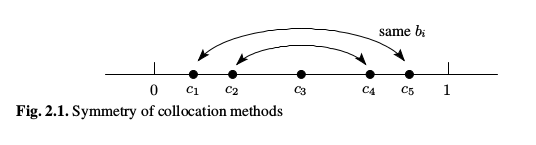
\includegraphics[width=.850\textwidth]{SymmetryCollocation}
 }
 \caption{ \small Kolokazio metodoen simetria.}
 \label{fig:pendulua}
 \end{figure}
  
\end{enumerate}

\paragraph{\textbf{Adibidea}.} $s=1$, $s=2$ eta $s=3$ ataletako Gauss metodoak.
\begin{equation*}
\begin{array}{c|c}
  \frac{1}{2} & \ \frac{1}{2} \\
  \hline
   & 1 \\
\end{array} \ \ \ ,  \ \ \ \ \ \ \ \ \
\begin{array}{c|c c}
  \frac{1}{2}-\frac{\sqrt{3}}{6} & \ \frac{1}{4} & \ \frac{1}{4}-\frac{\sqrt{3}}{6} \\
  \frac{1}{2}+\frac{\sqrt{3}}{6} & \ \frac{1}{4}+\frac{\sqrt{3}}{6} & \ \frac{1}{4} \\
  \hline
         &  \frac{1}{2} & \ \frac{1}{2} \\
\end{array}
\end{equation*}

\begin{equation*}
\begin{array}{c|c c c}
  \frac{1}{2}-\frac{\sqrt{15}}{10} & \ \frac{5}{36} & \ \frac{2}{9}-\frac{\sqrt{15}}{15} & \ \frac{5}{36}-\frac{\sqrt{15}}{30} \\
  \frac{1}{2}   & \ \frac{5}{36}+\frac{\sqrt{15}}{24} & \ \frac{2}{9} & \ \frac{5}{36}-\frac{\sqrt{15}}{24} \\
  \frac{1}{2}+\frac{\sqrt{15}}{10}   & \ \frac{5}{36}+\frac{\sqrt{15}}{30} & \ \frac{2}{9}+\frac{\sqrt{15}}{15} & \ \frac{5}{36} \\
  \hline
  & \frac{5}{18} & \ \frac{4}{9} & \ \frac{5}{18}
\end{array}
\end{equation*}

\paragraph*{}\emph{IRK} metodoetan, erronka handiena ekuazio-sistema ez-linealaren zenbakizko soluzio eraginkorra exekutatzea da. Nonstiff problemetarako, atalen hasieraketa ($Y_i^{[0]}$) egoki bat duen puntu-finkoko iterazioa erabil daiteke. Stiff problemetarako, puntu-finkoa iterazioak urrats tamaina txikiegia izatea behartuko luke eta ondorioz, Newton sinplifikatua erabili ohi da.         

\subsection*{IRK algoritmo orokorra.}


\begin{algorithm}[H]
 \BlankLine
  \For{$n\leftarrow 1$ \KwTo $endstep$}
  {
   \BlankLine
   Hasieratu  $Y_{i,n}^{[0]} \ \ , \ \ i=1,\dots,s $\;
    \BlankLine
   \While{ (konbergentzia lortu)}
   {
    \BlankLine 
    $F_{n,i}=f(Y_{n,i}) \ \ , \ \  i=1,\dots,s$\;
    $Y_{n,i}=y_{n-1}+ h \ \sum\limits_{j=1}^{s} a_{ij} F_{n,j}  \ \ , \ \  i=1,\dots,s$\;  
   }
   \BlankLine
    $y_{n}=y_{n-1}+ h \ \sum\limits_{i=1}^{s} b_i F_{n,i} $\;
   \BlankLine
 }
 \caption{Main Algorithm}
\end{algorithm}

\paragraph*{}Algoritmo nagusiko agindu bakoitzari ohar moduko egingo diogu, IRK metodoaren hainbat zehaztapen emateko helburuarekin.
\begin{enumerate}
\item Hasieratu  $Y_{i,n}^{[0]}$.

Atalen hasieraketa egokia definitu behar da. Aukera sinpleena $Y_{i,n}^{[0]}=y_{n-1}$ hasieratzea da baina aurreko urratseko informazioa erabiliz hurbilketa hobea lortu daiteke. Aurreko urratseko atalen polinomio interpolatzailearen bidezko hasieraketa era honetan adierazi dezakegu  $Y_{i,n}^{[0]}=g(Y_{i,n-1}) \ , \ i=1, \dots, s$.      

\item $F_{n,i}=f(Y_{n,i})$.

Atal bakoitzarentzat ekuazio diferentzialaren balioztapena independentea da eta modu paraleloan exekutatu daiteke.

\item   $Y_{n,i}=y_{n-1}+ h \ \sum\limits_{i=1}^{s} a_{ij} F_{n,j}  \ \ , \ \  i=1,\dots,s$.

Ekuazio-sistema ez lineala metodo iteratibo bat erabiliz askatu behar da. Metodo hau, Puntu-finkoaren metodoa edo Newton  sinplifikatuaren metodoa izan daiteke.  

\begin{enumerate}

\item Puntu-finkoko iterazioa.

\begin{algorithm}[H]
  \For{ (k=1,2,\dots)}
  {
   $Y_{i}^{[k]}=y_{n-1}+ h \ \sum\limits_{j=1}^{s} a_{ij} f(Y_i^{[k-1]}) $\; 
  }
 \caption{Main Algorithm}
\end{algorithm}


\item Newton sinplfifikatua.

Ekuazio-linealaren matrizea $M= I_s \otimes I_d -hA \otimes J, J=f'(y_n)$\$ definitzen dugu. Newton sinplifikatua puntu-finkoko iterazioa baino garestiagoa da, jakobiarra eta $M$ matrizearen \emph{LU-deskonposaketa} kalkulatu behar baititugu.  

\begin{algorithm}[H]
  $J=f'(y_n)$\;
  $M= I_s \otimes I_d -hA \otimes J$\;
  \For{ (k=1,2,\dots)}
  {
   $M\triangle Y^{[k-1]}=-F(Y^{k-1})$\;
   $Y^{[k]}=Y^{[k-1]}+\triangle Y^{[k-1]}$\; 
  }
 \caption{Main Algorithm}
\end{algorithm}


\end{enumerate}


\item $y_{n}=y_{n-1}+ h \ \sum\limits_{i=1}^{s} b_i F_{n,i} $\;

Integrazio luzeak direnean, urrats asko ematen dira eta koma higikorreko aritmetika dela eta, doitasun galera ekiditeko batura konpensatu teknika erabili ohi da.


\end{enumerate} 

\subsubsection*{Bigarren ordeneko ekuazio diferentzialak.}

Era honetako ekuazio diferentzialak ,

\begin{equation*}
\dot{u}=f(v), \ \ \dot{v}=g(u),
\end{equation*}

garrantzitsuak dira. Esaterako, bigarren ordeneko ekuazio diferentziala $\ddot{y}=f(y)$ eta Hamiltondar banagarriak $H(q,p)=T(p)+U(q)$ hauen kasu partikularra ditugu.

Runge-Kutta metodoaren ekuazioak era honetan bilakatzen dira,

\begin{equation*}
U_{i,n}=u_n+ \sum\limits_{i=1}^{s} a_{ij} f(V_{i,n})
\end{equation*}

\begin{equation*}
V_{i,n}=v_n+ \sum\limits_{i=1}^{s} a_{ij} g(U_{i,n})
\end{equation*}

Kasu honetan Gauss-Seidel iterazioa, puntu-finkoaren iterazio estandarra baino hobea da,

\begin{algorithm}[H]
  \For{ (k=1,2,\dots)}
  {
   $U_{i}^{[k+1]}=u_{n}+ h \ \sum\limits_{j=1}^{s} a_{ij} f(V_i^{[k]}) $\; 
   $V_{i}^{[k]}=v_{n}+ h \ \sum\limits_{j=1}^{s} a_{ij} g(U_i^{[k+1]}) $\; 
  }
 \caption{Main Algorithm}
\end{algorithm}
 
\paragraph*{}Bigarren ordeneko ekuazio diferentzialak ditugunean,
\begin{equation*}
\dot{u}=f(v), \ \ \dot{v}=u,
\end{equation*}

Gauss-Seidel iterazioa honakoa dugu,

\begin{algorithm}[H]
  \For{ (k=1,2,\dots)}
  {
   $V_{i}^{[k+1]}=v_{n}+h c_i v_{n}+ h^2 \ \sum\limits_{j=1}^{s} \tilde{a}_{ij} f(V_i^{[k]}) $\;  
  }
 \caption{Main Algorithm}
\end{algorithm} 


 

\subsection{Kolokazio metodoak.}

Kolokazio metodoak ekuazio diferentzialen zenbakizko soluzioa azaltzeko beste modu bat dira. Gauss metodoak kolokazio metodoak ditugu eta hauen abantaila da, zenbakizko soluzioa diskretizazio puntuetan ez ezik, polinomio interpolatzaile batek modu jarraian emandako soluzioa adierazten duela. Honako definizioa emango dugu,

\begin{definizioa}
$c_1,c_2,\dots,c_s \ \ (0\leq c_i \leq 1)$ zenbaki errealak izanik, $s$-mailako $u(t)$   kolokazio polinomioak honakoa betetzen du,

\[u(t_0)=y_0 ,\]
\[\dot{u}(t_0+c_ih)=f(t_0+c_i h, u(t_0+c_i h)), \ \ i=1,\dots,s.\] 


Orduan soluzioa $y_1=u(t_0+h)\approx y(t_0+h)$ da..
\end{definizioa}

\begin{teorema}
\textbf{Theorem 1.4 (Guillou and Soule 1969, Wright 1970).}
Kolokazio metodoaren definizioa eta jarraian emandako moduan kalkulatutako koefizienteko s-ataleko Runge-Kutta metodoa baliokideak dira.

\begin{equation}
a_{ij}=\int_{0}^{c_i} l_j(\tau) \ d\tau, \ \ b_i=\int_{0}^{1} l_i(\tau) \ d\tau
\end{equation}

non $l_i(\tau)$ Lagrangiar polinomioa dugu $l_i(\tau)=\prod_{l\neq i} \frac{(\tau-c_l)}{(c_i-c_l)}$.
\end{teorema}

\paragraph{\textbf{Definizioa}.} Gauss metodoak $c_i$ ($1 \leq i \leq s)$ koefizienteak "sth shifted Legendre" polinomioaren zeroak aukeratuz,

\begin{equation*}
\frac{d^s}{dx^s} \big(x^s(x-1)^s \big),
\end{equation*} 

Nodo hauetan oinarritutako Runge-Kutta metodoa $p=2s$ ordena du.

\begin{figure}[h]
\centering
\subfloat[kolokazio metodoak.]{
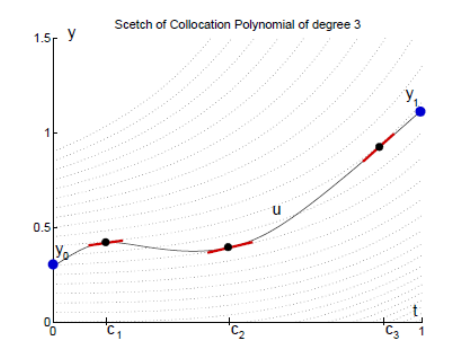
\includegraphics[width=.450\textwidth]{KolokazioMetodoa}
}
\caption{ \small kolokazio metodoak.}
\label{fig:kolokazio metodoak}
\end{figure}


\paragraph*{} Gauss metodoaren koefizienteak kalkulatzeko bi aukera ditugu. Lehen aukera,  \emph{Mathematicak} NDSolve paketean inplementatuta dagoen koefizienteak kalkulatzeko funtzioa: ImplicitRungeKuttaGaussCoefficients[]. Bigarren aukera, guk koefizienteak kalkulatzeko garatutako funtzioa erabiltzea.  

\begin{lstlisting} [language=Mathematica]

GaussCoefficients[s_Integer, doi_, a_Symbol, b_Symbol, c_Symbol] :=
    Module[{f, g, ff, glist, B, A},
 
         Do[c[i] = N[(Root[LegendreP[s, #] &, i] + 1)/2, doi] // Simplify, {i, s}
           ];
         ff = Collect[InterpolatingPolynomial
                     [Table[{c[i], f[i]}, {i, s}], x], f[_]];
         glist = Table[g[i] = Collect[ff, f[_],
                                      Simplify[\!\(\*SubsuperscriptBox[\(\[Integral]\), \(0\), \(c[
          i]\)]\(#1 \[DifferentialD]x\)\)] &], {i, 1, s}];
               yy = Collect[ff, f[_], Simplify[\!\(
\*SubsuperscriptBox[\(\[Integral]\), \(0\), \(1\)]\(#1 \
\[DifferentialD]x\)\)] &];
                B = Table[b[i] = \!\(
\*SubscriptBox[\(\[PartialD]\), \(f[i]\)]yy\), {i, 1, s}];
               
 A = Table[a[i, j] = D[g[i], f[j]], {i, 1, s}, {j, 1, s}];
         {Array[c, s], B, A}
 ]

\end{lstlisting}


\section{Konposizio metodoak.}

\subsection{Sarrera.}

Konposizio metodoak, oinarrizko metodo bat edo gehiago konposatuz eraikitako zenbakizko integrazio metodoak dira.  Oinarrizko metodoekin segidan exekutatutako azpi-urrats kopuru batek, konposizio metodoaren integrazioaren urrats bat osatzen du. Helburua orden baxuko metodo batetik abiatuta, orden altuko metodoa eraikitzea da; konposizio metodoak automatikoki konposatutako metodoaren propietateak (simetri, sinplektikoa,\dots) jasotzen ditu. 

\paragraph*{\textbf{Definizioa orokorra}.}
$\phi_h$ oinarrizko metodoa eta $\gamma_1,\dots,\gamma_s$ zenbaki errealak emanik, urrats luzera hauen $\gamma_1 h,\gamma_2 h,\dots,\gamma_s h$ konposaketari dagokion konposizio metodoa,
\begin{equation}
\Psi_h=\phi_{\gamma_s h} \circ \dots \circ \phi_{\gamma_{1 h}}.
\end{equation}

\paragraph*{\textbf{Teorema}.}
Demagun $\phi_h$ urrats bakarreko eta $p$ ordeneko metodoa. Konposizio metodoa gutxienez $p+1$ ordeneko izango da baldin,
\[\gamma_1+\dots+\gamma_s=1,\] 
\begin{equation}
\gamma_1^{p+1}+\dots+\gamma_s^{p+1}=0.
\end{equation}

\paragraph*{\textbf{Algoritmoa}.}
Konposizio metodoen algoritmo orokorra honakoa izango litzateke:

\begin{algorithm}[H]
 \BlankLine
  \For{$n\leftarrow 1$ \KwTo $endstep$}
  {
   \BlankLine
    $Y_{0,n}=y_{n-1} $\;
    \BlankLine
   \For{i=1,2,...,s}
   {
    \BlankLine 
    $Y_{i,n}=\phi_{\gamma_i h}(Y_{i-1,n})$\;
   }
   \BlankLine
    $y_{n}=Y_{s,n}$\;
   \BlankLine
 }
 \caption{Konposizio metodoak.}
\end{algorithm}
 
\paragraph*{Oharrak.}
Konposizio metodoei buruzko hainbat ohar azpimarratuko ditugu:
\begin{enumerate}
\item{Esplizitua.}

Konposizio metodo hauek esplizituak dira. Metodo hauetan ez da ekuazio sistemarik askatu behar, eta kalkuluak azkarrak dira. 

\item{Sekuentziala.}

Urrats bakoitzaren kalkuluak modu sekuentzialean egin behar ditugu.

\item{Memoria gutxi.}

Ez da tarteko baliorik gorde behar eta datu-egitura berezirik memorian gorde behar.   

\item{Oinarrizko metodoa: Störmer-Verlet.}

Bigarren ordeneko ekuazio diferentzialak ditugunean, Störmer-Verlet integratzailean oinarritzen diren konposizio metodoekin urrats bakoitzean $s$ ekuazio diferentzialaren balioztapena egin behar ditugu.

\end{enumerate}


\paragraph*{} Konposizio metodo eraginkorra $s$-atal gutxirekin, $p$ orden altuko metodoa dugu. Sofronio eta Spalettaren ($2004$), $s=35$ eta $p=10$ ordeneko metodoa \cite{Sofroniou2005}, orain arteko lortutako orden altueneko konposizio metodo eraginkorrena kontsideratu daiteke. \emph{IRK} metodoa konposizio metodo honekin alderatuko dugu eta beraz, jarraian modu laburrean konposizio metodo hau azalduko dugu.     

\subsection{CO1035: $10$ ordeneko konposizio metodoa.}

Konposizio metodo simetrikoa da. Oinarrizko metodoa simetrikoa eta $p=2$ dela baliatuz eraikitako metodoa da. 

\begin{table}
\caption[C01035 konposizio metodoa.] 
{\small{10 ordeneko metodoa konposizio metodoa (CO1035).}}
\label{tab:31}       % Give a unique label
\begin{tabular}{ c c } 
 \hline
 Koefiziente         &  Balioa \\
 \hline
 $\gamma_1=\gamma_{35}$ & 0.07879572252168641926390768 \\
 $\gamma_2=\gamma_{34}$ & 0.31309610341510852776481247 \\ 
 $\gamma_3=\gamma_{33}$ & 0.02791838323507806610952027 \\
 $\gamma_4=\gamma_{32}$ &-0.22959284159390709415121340 \\ 
 $\gamma_5=\gamma_{31}$ & 0.13096206107716486317465686 \\ 
 $\gamma_6=\gamma_{30}$ & -0.26973340565451071434460973 \\ 
 $\gamma_7=\gamma_{29}$ & 0.07497334315589143566613711 \\ 
 $\gamma_8=\gamma_{28}$ & 0.11199342399981020488957508 \\ 
 $\gamma_9=\gamma_{27}$ & 0.36613344954622675119314812 \\ 
 $\gamma_{10}=\gamma_{26}$ & -0.39910563013603589787862981 \\ 
 $\gamma_{11}=\gamma_{25}$ & 0.10308739852747107731580277 \\
 $\gamma_{12}=\gamma_{24}$ & 0.41143087395589023782070412 \\ 
 $\gamma_{13}=\gamma_{23}$ & -0.00486636058313526176219566 \\ 
 $\gamma_{14}=\gamma_{22}$ & -0.39203335370863990644808194 \\ 
 $\gamma_{15}=\gamma_{21}$ & 0.05194250296244964703718290 \\ 
 $\gamma_{16}=\gamma_{20}$ & 0.05066509075992449633587434 \\ 
 $\gamma_{17}=\gamma_{19}$ & 0.04967437063972987905456880 \\ 
 $\gamma_{18}$ & 0.04931773575959453791768001 \\ 
  \hline
 \end{tabular}
\end{table}


\paragraph*{\textbf{Gure inplementazioa.}} Gure abiapuntua Haireren konposizio metodoaren Fortran kodea izan da. Konposizio metodoaren azalpenak liburuko \cite{Hairer2006}  \emph{II.4} eta \emph{V.3} ataletan ematen ditu. \emph{GNI-Comp} izeneko kodea eskuragarri dago \cite{HairerGniComp} helbidean. Kodearen C-lengoaiako bertsioa garatu dugu.

\paragraph*{}$\phi_h$ metodoa $p=2$ ordenekoa eta simetrikoa izanik, era honetako konposizioak aurkitu dira,
\begin{equation}
\Psi_h=\phi_{\gamma_s h} \circ \phi_{\gamma_s-1 h} \circ \dots \circ \phi_{\gamma_{2 h}} \circ \phi_{\gamma_{1 h}} 
\end{equation}
non $\gamma_s=\gamma_1, \gamma_{s-1}=\gamma_2,\dots$ 


\paragraph*{\textbf{Koefizienteak}.}

Konposizio metodoaren oinarrizko metodoa \emph{Stömer-Verlet}  $\phi_h=\varphi_{h/2}^{1} \circ \varphi_{h}^{2} \circ \varphi_{h/2}^{1}$  dugula kontutan hartuta,

\begin{equation*}
\Psi_h=(\varphi_{h \gamma_s/2}^{1} \circ \varphi_{h \gamma_s}^{2} \circ \varphi_{h \gamma_s/2}^{1}) \circ \dots 
       \circ
       (\varphi_{h \gamma_2/2}^{1} \circ \varphi_{h \gamma_2}^{2} \circ \varphi_{h \gamma_2/2}^{1}) 
       \circ
       (\varphi_{h \gamma_1/2}^{1} \circ \varphi_{h \gamma_1}^{2} \circ \varphi_{h \gamma_1/2}^{1})  
\end{equation*}

\paragraph*{}Beraz jarraian dauden $\varphi^1$ fluxuak elkartuz,

\begin{equation*}
\Psi_h=\varphi_{h a_{s+1}}^{1} \circ \varphi_{h b_s}^{2} \circ \dots 
       \circ
       \varphi_{h a_3} \circ \varphi_{h b_2}^{2} 
       \circ
       \varphi_{h a_2}^{1} \circ \varphi_{h b_1}^{2} \circ \varphi_{h a_1}^{1}  
\end{equation*}

non $a_1=a_{s+1}=\gamma_1/2$, $b_i=\gamma_i$, $a_k=(\gamma_k+\gamma_{k-1})/2$, $i=1,\dots,s$ eta $k=2,\dots,s$.

\paragraph*{}Tarteko urratsetan, lehen atala $\varphi_{h a_1}^{1}$ eta azkena $\varphi_{h a_1}^{1}$ bakar batean elkar daitezke, 

\begin{equation*}
\Psi_h=\varphi_{h 2 a_{s+1}}^{1} \circ \varphi_{h b_s}^{2} \circ \dots 
       \circ
       \varphi_{h a_3} \circ \varphi_{h b_2}^{2} 
       \circ
       \varphi_{h a_2}^{1} \circ \varphi_{h b_1}^{2}.
\end{equation*}

\section{Splitting metodoak.}

\subsection{Sarrera.}

\emph{Splitting metodoak}, bektore eremua $f: \mathbb{R}^d \rightarrow \mathbb{R}^d$ sistema osoa integratzeko baino errazagoa diren azpiproblemetan, $f^{[i]}$ ($f=\sum\limits_{i=1}^{m} f^{[i]}$), deskonposatu daitezkeen ekuazio diferentzialetarako zenbakizko integrazioak dira.  

\paragraph*{}Maiz, jatorrizko $\dot{\mathbf{y}}=\mathbf{f}(\mathbf{y})$ problema era honetan bana daiteke,
\begin{equation}
\dot{\mathbf{y}}=\mathbf{f^{[1]}}(\mathbf{y})+\mathbf{f^{[2]}}(\mathbf{y}),
\end{equation} 
non $\dot{\mathbf{y}}=\mathbf{f^{[1]}}(\mathbf{y})$ eta $\dot{\mathbf{y}}=\mathbf{f^{[2]}}(\mathbf{y})$ sistemen fluxu zehatzak, $\varphi_t^{[1]}$ eta $\varphi_t^{[2]}$ esplizituki kalkula daitezkeen. 

\paragraph*{\textbf{Lie-Trotter splitting}.}
$p=1$ ordeneko metodoak,
\begin{equation}
\phi_h = \varphi_h^{[1]} \circ \varphi_h^{[2]} \ \ \ edo \ \ \ \phi_h^{*} = \varphi_h^{[2]} \circ \varphi_h^{[1]} .
\end{equation}

\paragraph*{\textbf{Strang-Marchuk splitting}.}
$p=2$ ordeneko metodo simetrikoa,
\begin{equation}
\phi_h =  \varphi_{\frac{h}{2}}^{[1]} \circ \varphi_h^{[2]} \circ \varphi_{\frac{h}{2}}^{[1]}
\end{equation} 

\paragraph*{\textbf{Splittig metodo orokorrak}.}
Konposizio metodoen modu berean, oinarrizko Splitting metodoak konposatuz orden altuagoko metodoak lortzen dira, 

\begin{equation}
\Psi_h=\varphi^{[1]}_{a_{s+1} h} \circ \varphi^{[2]}_{b_s h} \circ \varphi^{[1]}_{a_s h} \circ \dots \circ \varphi^{[1]}_{a_2 h} \circ \varphi^{[2]}_{b_1 h} \circ \varphi^{[1]}_{a_1 h}.
\end{equation}

\paragraph*{} $a_i,b_i$ koefizienteek metodoaren ordena definitzen dute. Metodoa simetrikoa bada $\Psi_h=\Psi_h^{*}$,

\begin{equation*}
a_1=a_{s+1}, \ b_1=b_{s}, \ a_2=a_s, b_2=b_{s-1}, \dots
\end{equation*} 

\paragraph*{\textbf{Algoritmoa}.}
\emph{Splitting metodoen} algoritmo orokorra honakoa izango litzateke:

\begin{algorithm}[H]
 \BlankLine
  \For{$n\leftarrow 1$ \KwTo $endstep$}
  {
   \BlankLine
    $Y_{0,n}=y_{n-1} $\;
    \BlankLine
   \For{i=1,2,...,s}
   {
    \BlankLine 
    $Y_{i,n}=(\varphi^{[2]}_{b_i h} \circ \varphi^{[1]}_{a_i h})(Y_{i-1,n})$\ ;
   }
   \BlankLine
    $y_{n}=Y_{m,n}$\;
   \BlankLine
 }
 \caption{Splitting metodoak.}
\end{algorithm}

\paragraph*{Oharrak.}
Splitting metodoen algoritmoan, konposizio metodoen algoritmoei buruzko ezaugarri berdinak errepikatu beharko genituzke. 

\paragraph*{\textbf{Fluxu zehatza eta zenbakizko fluxua konbinatuz}.}
Demagun sistema $\dot{\mathbf{y}}=\mathbf{f}(\mathbf{y})$ era honetan banatzen dugula,
\begin{equation}
\dot{\mathbf{y}}=\mathbf{f^{[1]}}(\mathbf{y})+\mathbf{f^{[2]}}(\mathbf{y}),
\end{equation} 

Suposatu bakarrik $\dot{\mathbf{y}}=\mathbf{f^{[1]}}(\mathbf{y})$ sistemaren fluxua zehatza $\varphi_t^{[1]}$ kalkulatu daitekeela eta $\phi_t^{[2]}$, $\dot{\mathbf{y}}=\mathbf{f^{[2]}}(\mathbf{y})$ sistemari aplikatutako zenbakizko integrazio dugula. Orduan konposizio metodoaren oinarrizko metodoa honakoa kontsideratu daiteke,

\begin{equation*}
\phi_h=\varphi_h^{[1]} \circ \phi_h^{[2]}, \ \ \ \ \ \  \phi_h^{*}=\phi_h^{[2]*} \circ \varphi_h^{[1]}.
\end{equation*}


\paragraph*{} \emph{} Splitting metodoak konposizio metodoen interpretazioa emanez,
\begin{equation}
\Psi_h=\varphi^{[1]}_{a_{s} h} \circ \phi^{[2]}_{a_s h} \circ \phi^{[2]*}_{b_s h} \circ \varphi^{[1]}_{(b_s+a_s-1) h} \circ \phi^{[2]}_{a_s h} \circ \dots  \circ \phi^{[2]*}_{b_1 h} \circ \varphi^{[1]}_{b_1 h}.
\end{equation}


\subsection{Eguzki-sistemari egokitutako splitting metodoak.}

Honakoa dugu N-gorputzeko problema grabitazionalaren Hamiltondarra,
\begin{equation*}
H(p,q)=T(p)+U(q).
\end{equation*}

Bi koordenatu sistema (\emph{Jacobi} edo koordenatu Heliozentrikoak) erabiliaz,  Hamiltondarra beste modu honetan berridatzi daiteke,
\begin{equation*}
H=H_K+H_I,  \ \ |H_I|\ll|H_K|,
\end{equation*}
non alde nagusia $H_K$ planeta bakoitzaren eguzki inguruko mugimendu kepleriarra den eta $H_I$ aldiz, planeten arteko interakzioek eragiten duten perturbazio txikia.    

\paragraph*{}Eguzki-sistemaren N-gorputzeko problema grabitazionalari egokitutako zenbakizko bi integratzaile sinplektiko azalduko ditugu. Lehena, J.Laskarrek eta P.Robutelek \cite{Laskar2001} definitutako \emph{$SABAC_4$} integratzailea eta bigarrena, Blanes-ek \cite{Blanes2013} \cite{Farres2013} definitutako \emph{$ABAH1064$} integratzailea. 

\begin{enumerate}
\item Laskarren ($2001$) $SABAC_4$ zenbakizko integratzailea \cite{Laskar2001}.
$SABA_4$ integratzailea definitzen duten koefizienteak (taula \ref{tab:32}).
 
\begin{table}
\caption[$SABA_4$ splitting metodoa.] 
{\small{$SABA_4$ splitting metodoa.}}
\label{tab:32}       % Give a unique label
\begin{tabular}{ c c | c c} 
 \hline
 Koefiziente         &  Balioa  & Koefiziente         &  Balioa  \\
 \hline
 $c_1$ & $\frac{1}{2}-\frac{\sqrt{525+70\sqrt{30}}}{70}$ 
       & $d_1$ & $\frac{1}{4}-\frac{\sqrt{30}}{72}$\\
 $c_2$ & $\frac{\big( \sqrt{525+70 \sqrt{30}}-\sqrt{525-70 \sqrt{30}} \big)}{70}$ 
       & $d_2$ & $\frac{1}{4}+\frac{\sqrt{30}}{72}$\\
 $c_3$ & $\frac{\sqrt{525-70\sqrt{30}}}{35}$ & & \\
  \hline
 \end{tabular}
\end{table}


\paragraph*{Hamiltondarra.} $H=H_A+\epsilon H_B$ izanik eta goiko notazioa erabiliz,

\begin{equation*}
SABA_4=\varphi^{[A]}_{c_1 h} \circ \varphi^{[B]}_{d_1 h} \circ \varphi^{[A]}_{c_2 h} \circ \varphi^{[B]}_{d_2 h}
         \circ  \varphi^{[A]}_{c_3 h}   \circ
          \varphi^{[B]}_{d_2 h} \circ \varphi^{[A]}_{c_2 h} \circ   \varphi^{[B]}_{d_1 h}\circ  \varphi^{[A]}_{c_1 h}.
\end{equation*}


\paragraph*{Corrected integrator.}

Urrats bat gehitutako integratzailea $SABAC_4$,

\begin{equation*}
SABAC_4=\varphi{[B]}_\frac{-c}{2} \circ SABA_4 \circ \varphi{[B]}_\frac{-c}{2},
\end{equation*}
non $c=0.003396775048208601331532157783492144$.\\

\item. $ABAH1064$ (Blanes, 2013).

\paragraph*{}Eguzki sistemaren integraziorako koordenatu Heliozentrikoei dagokion Hamiltondarra era honetakoa dugu,
\begin{equation*}
H(p,q)=H_K(p,q)+H_I(p,q), \ \ H_I(p,q)=T_1(p)+U_1(q). 
\end{equation*}

$H_I(p,q)$ fluxua zehazki kalkulatu ordez honen hurbilpen bat erabiliko dugu,
\begin{equation*}
\varphi_t^I \approx \tilde{\varphi}_t^I= \varphi_{\frac{tb_i}{2}}^{[U_1]} \circ \varphi_tb_i^{[T_1]} \circ \varphi_{\frac{tb_i}{2}}^{[U_1]}.
\end{equation*}

$ABAH1064$, $p=10$ eta $s=9$ splitting metodoa aztertuko dugu,
\begin{equation*}
ABAH1064=\prod\limits_{i=1}^{s} \varphi_{a_ih}^K \circ \tilde{\varphi}_{b_ih}^I
\end{equation*}
non $a_i$,$b_i$ koefizienteak beheko taulan (taula \ref{tab:33}) definitzen diren.  

\begin{table}
\caption[$ABAH1064$ splitting metodoa.] 
{\small{$ABAH1064$ splitting metodoa.}}
\label{tab:33}       % Give a unique label
\begin{tabular}{ c c } 
 \hline
 Koefiziente         &  Balioa \\
 \hline
 $a_1=a_9$ & $0.04731908697653382270404371796320813250988$ \\
 $a_2=a_8$ & $0.2651105235748785159539480036185693201078$ \\
 $a_3=a_7$ & $-0.009976522883811240843267468164812380613143$ \\
 $a_4=a_6$ & $-0.05992919973494155126395247987729676004016$ \\
 $a_5$ & $0.2574761120673404534492282264603316880356$ \\
 $b_1=b_9$ & $0.1196884624585322035312864297489892143852$ \\
 $b_2=b_8$ & $0.3752955855379374250420128537687503199451$ \\
 $b_3=b_7$ & $-0.4684593418325993783650820409805381740605$ \\
 $b_4=b_6$ & $0.3351397342755897010393098942949569049275$ \\
 $b_5$ &  $0.2766711191210800975049457263356834696055$ \\
  \hline
 \end{tabular}
\end{table}

\end{enumerate} 


\section{Kepler fluxua.}

\paragraph*{\textbf{Bi gorputzen problema}.} Kepler problemari dagokion Hamiltondarra,
\begin{equation}
H(\bf{p},\bf{q})=\frac{\mathbf{p}^2}{2m}-\frac{\mu}{\|\mathbf{q}\|}.
\end{equation}

\paragraph*{} Elkar erakartzen diren bi gorputzen mugimendua kalkulatzeko, gorputz baten kokapena koordenatu sistemaren jatorria kontsideratuko dugu. Honen arabera, $m=(1/m_1+1/m_2)^{-1}$ eta $\mu=Gm_1m_2$ definituko ditugu. 

Hamiltondarrari dagokion bigarren ordeneko ekuazio diferentzialak,

\begin{equation}
\ddot{\mathbf{q}}= - \frac{k\mathbf{q}}{\|\bf{q}\|^3} ,
\end{equation}
non $k= \mu / m$ eta  $\mathbf{q}\in \mathbb{R}^3$.


\paragraph*{\textbf{Ideia nagusia}.} Koordenatu cartesiarretatik koordenatu eliptikoetara $(a,e,i,\Omega,E)$ itzulpena egingo dugu. Kontutan hartuta $E$ (izena??) aldagai ezik beste aldagaiek konstante mantentzen direla, $E_0$ abiapuntua harturik, $\triangle t$ denbora tartea aurrera egingo dugu $E_1$ balioa berria kalkulatzeko. Azkenik, koordenatu eliptikoetatik koordenatu cartesiarrak berreskuratuko ditugu kokapen eta abiadura berriekin. 

\begin{equation*}
(\bf{q_0},\bf{v_0}) \in \mathbb{R}^6 \ \ \ \longrightarrow \ \ \  (a,e,i,\Omega,E_0) \in \mathbb{R}^6 
\end{equation*}

\begin{equation*}
\downarrow \triangle t
\end{equation*}

\begin{equation*}
(\bf{q_1},\bf{v_1}) \in \mathbb{R}^6 \ \ \ \longleftarrow \ \ \  (a,e,i,\Omega,E_1) \in \mathbb{R}^6 
\end{equation*}

\paragraph*{\textbf{Newton metodoa}.} Kepler-en ekuazioan oinarrituz ($E-e\sin E=n (t-t_p)$),  $E_1=\triangle E+E_0$ balioa kalkulatuko Newtonen metodoa aplikatuz,

\begin{equation*}
f(\triangle E)=\triangle E - ce \sin(\triangle E)- se (\cos(\triangle E)-1)-n \triangle t=0
\end{equation*}
\begin{equation}
\triangle E^{[k+1]}=\triangle E^{[k]}- \frac{f(\triangle E^{[k]})}{f'(\triangle E^{[k]})}
\end{equation}

\paragraph*{\textbf{Ekuazioak}.} Gure inplementazioan erabilitako ekuazio guztien azalpenak eta definizoak eranskinean eman ditugu.

\section{Laburpena.}

Hauek dira Eguzki sistemaren integraziorako konparatuko ditugun metodoak,

\begin{table}{htb}
\caption{Integrazio metodoen laburpena}
\label{tab:1}       % Give a unique label
\begin{tabular}{ c|c c c } 
           &  C1035             &  ABAH1064           & GAUSS-12           \\
 \hline
 	       & Konposizio met.    & Splitting met.     & IRK met.            \\
 	       & Sofronio (2004)    & Blanes et al. 2013 &                     \\
 \hline 
               &                    &                    &                 \\
 Hamiltoniarra & Orokorra           & Perturbatua        & Orokorra        \\ 	    
 Mota          & Esplizitua         & Esplizitua         & Inplizitua      \\ 
 Ordena        & 10                 & 10                 & 12              \\ 
 Atalak        & 35                 & 9                  & 6               \\ 
 Parall.       & Ez                 & Ez                 & Bai             \\  
\end{tabular}
\end{table}
 
